This chapter describes the implementation of the cached profiles functionality for HotSpot, written as part of this thesis.
HotSpot is vital part of the open source project \texttt{OpenJDK} and the source code is available at \url{http://openjdk.java.net/}.
\\\\
Most of the code additions are included in two new classes \texttt{/share/vm/ci/ciCacheProfiles.cpp} and \\\texttt{/share/vm/ci/ciCacheProfilesBroker.cpp} as well as significant changes to \texttt{/share/vm/ci/ciEnv.cpp} and \texttt{/share/vm/compiler/compileBroker.cpp}.
\\
The core functionality is located in \texttt{/share/vm/ci/ciCacheProfiles.cpp}, a class that takes care of setting up the cached profile datastructure as well as providing public methods to check if a method is cached or not. The class \texttt{/share/vm/ci/ciCacheProfilesBroker.cpp} is used before a cached method gets compiled. It is responsible for setting up the compilation environment, so the JIT compiler can use the cached profiles.
\\\\
A full list of modified files and the changes can be seen in the webrev at \url{http://mohlerm.ch/b/webrev.01/} or Appendix \ref{a:codechanges}.
The changes are provided in form of a patch for HotSpot version 1aef080fd28d. In the following, the original version is referred to as \textit{baseline}.
\\\\
I will describe and explain the functionality and the implementation design decision in the following sections, ordered by their execution order.

\section{Creating cached profiles}
\label{s:creatingprofiles}
The baseline version of HotSpot already offers a functionality to replay a compilation based on previously saved profiling information.
This is mainly used in case the JVM crashes during a JIT compilation to replay the compilation process and allow the JVM developer to further investigate the cause of this incident.
Apart from this automatic process there exists the possibility to invoke the profile saving manually by specifying the \texttt{DumpReplay} compile command option per method.
\\\\
I introduce a new method option called \texttt{DumpProfile} as well as a new compiler flag \newline\texttt{-XX:+DumpProfiles} that appends profiling information to a file as soon as a method gets compiled. The first option can be specified as part of the \texttt{-XX:CompileCommand} or \texttt{-XX:CompileCommandFile} flag and allows the user to select single methods to dump their profile. The second commands dumps profiles of all compiled methods.
The profile get converted to a string and saved in a simple text file, which is called \textit{cached\_profiles.dat}.
\\\\
The system will only consider compilations of Level 3 or Level 4. Level 1 and Level 2 are rarely used in practice and do only include none or little profiling information.
\\\\
Each of these dumped strings of compilation data consists of multiple \texttt{ciMethod} entries, \texttt{ciMethodData} entries and one compile entry. They are separated by linebreaks and keywords make sure the data can be parsed correctly. A shortened example of a cached profile can be found in Appendix \ref{a:cacheprofileexample}. The \texttt{ciMethod} entries contain information about the methods used in the compilation and Table \ref{t:cimethod} describes it in more detail. The \texttt{ciMethodData} (see Table \ref{t:cimethoddata}) includes all profiling data about the methods itself to be able to redo the compilation.
The compile entry saves the bytecode index in case of OSR, the level of the compilation and lists all inlining decisions (Table \ref{t:compile}).
\\\\
Since method often get compiled multiple times and at different tier, this results in dumping compilation information about the same method multiple times. This is intentional and is taken care of when loading the profiles (also see Section \ref{s:initializingprofiles}).
\begin{table}[ht!]
  \caption{content of ciMethod entry in cached Profile}
  \label{t:cimethod}
  \begin{center}
    \begin{tabular}{|p{5cm}|p{10.5cm}|} 
      \hline
       \textbf{name} & \textbf{description} \\ \hline\hline
       class\_name,& used to identify the method\\
       method\_name, & \\
       signature & \\ \hline
       invocation\_counter & number of invotations\\ \hline
       backedge\_counter & numbe of counted backedges\\ \hline
       interpreter\_invocation\_count & number of invocations during interpreter phase\\ \hline
       interpreter\_throwout\_count & how many times method was exited via exception while interpreting\\ \hline
       instructions\_size\_name & rough size of method before inlining\\ \hline
    \end{tabular}
  \end{center}
\end{table}
\begin{table}[ht!]
  \caption{content of ciMethodData entry in cached Profile}
  \label{t:cimethoddata}
  \begin{center}
    \begin{tabular}{|p{5cm}|p{10.5cm}|} 
      \hline
       \textbf{name} & \textbf{description} \\ \hline\hline
       class\_name,& used to identify the method\\
       method\_name, & \\
       signature & \\ \hline
       state & if data is attached and matured\\ \hline
       current\_mileage & maturity of the oop when snapshot is taken\\ \hline
       orig &  snapshot of the original header\\ \hline
       data & the actual profiling data\\ \hline
       oops & ordinary object pointers, JVM managed pointers to object\\ \hline        
    \end{tabular}
  \end{center}
\end{table}
\begin{table}[ht!]
  \caption{content of compile entry in cached Profile}
  \label{t:compile}
  \begin{center}
    \begin{tabular}{|p{5cm}|p{10.5cm}|} 
      \hline
       \textbf{name} & \textbf{description} \\ \hline\hline
       class\_name,& used to identify the method\\
       method\_name, & \\
       signature &\\ \hline
       entry\_bci & byte code index of method\\ \hline
       comp\_level & compilation level of record\\ \hline
       inline & array of inlining information\\ \hline        
    \end{tabular}
  \end{center}
\end{table} 
\section{Initializing cached profiles}
\label{s:initializingprofiles}
The information dumped in step \ref{s:creatingprofiles} can now be used in a next run of that particular program.
To specify that profiles are available, I introduce a new compiler flag \texttt{-XX:+CacheProfiles} that enables the use of previously generated profiles. Per default it reads from a file called \textit{cached\_profiles.dat} but a different file can be specified using \\\texttt{-XX:CacheProfilesFile=other\_file.dat}.
\\\\
Before any cached profiles can be used the virtual machine has to parse that file and organize the profiles and compile information in a datastructure. This datastructure is kept in memory completely during the whole execution of the JVM to avoid multiple disk accesses.
The parsing process gets invoked during boot up of the JVM, directly after the compileBroker gets initialized. This happens before any methods get executed and blocks the JVM until finished.
\\\\
As mentioned in Section \ref{s:creatingprofiles} the file consists of method informations, method profiles and additional compile information. The parser scans the file once and creates a so called \texttt{CompileRecord} for each of the methods that include compilation information in the file. This compile record also includes the list of method information (\texttt{ciMethod}) and their profiling information (\texttt{ciMethodData}).
As mentioned previously, a method's compile information could have been dumped multiple times, so it can happen that there are multiple \texttt{CompileRecords} for the same method. In this case, HotSpot will only keep the \texttt{CompileRecords} that are created based on the last data written to the file.
Since profiling information only grow, the compilation that happened last contains the richest profile and is considered the best.
This is based on the fact that the richer the profile the more information about the method execution is known and influences the compiled version of that method. For example, a profile for a method might include data for all its branches and can therefore avoid running into uncommon traps and trigger deoptimizations.
\\\\
The \texttt{CompileRecord} as well as the lists of methods information and profiles are implemented as an array located in HotSpot's heap space.
They get initialized with a length of 8 and grow when needed. This implementation choice has been done for simplicity and leaves up room for further optimizations.

\section{Using cached profiles}
\label{s:usingprofiles}
The thesis offers three different modes \texttt{mode 0}, \texttt{mode 1} and \texttt{mode 2} on how the profiles are used.
The following paragraph describes the behaviour of \texttt{mode 0} and \texttt{mode 1} and I will discuss the differences in detail in Section \ref{s:cacheprofilesmode}, especially \texttt{mode 2} in Section \ref{s:mode2}.
\\\\
The idea is to use cached profiles whenever possible and if none are available continue as usual.
A graphical, simplified overview of the program flow for compiling a method with the changes introduced in this thesis can be found in Figure \ref{f:programflow}.
\begin{figure}[h]
  \begin{center}
    \centering
    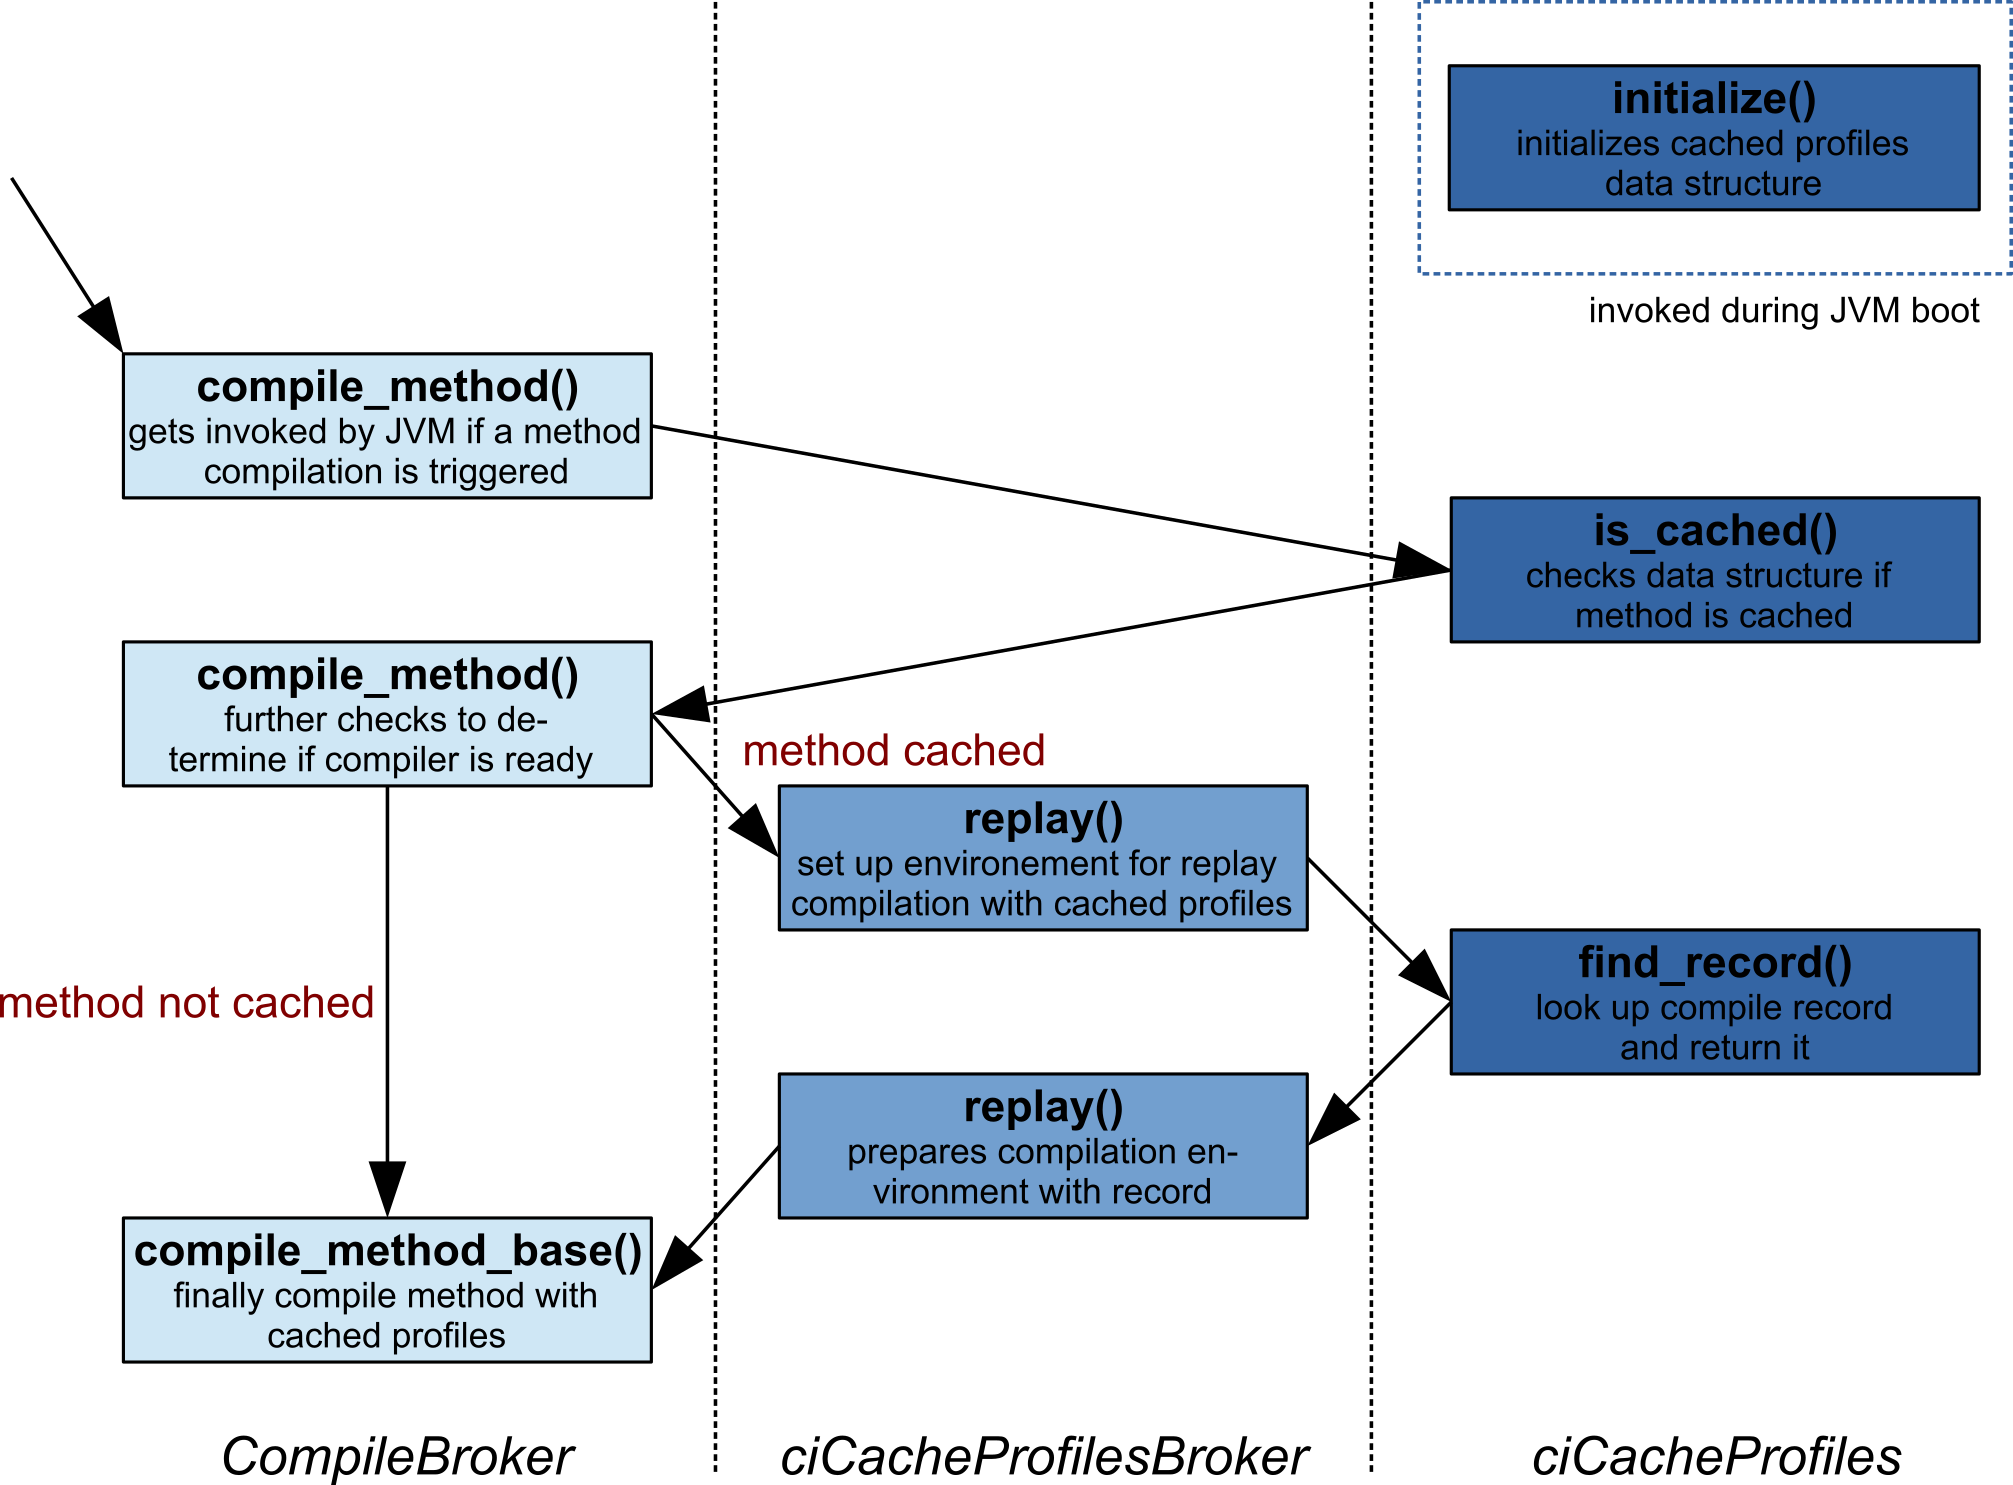
\includegraphics[width=0.8\textwidth]{figures/program_flow.png}
    \caption{program flow for compiling a method}
    \label{f:programflow}
  \end{center}
\end{figure}
As mentioned before, once certain thresholds are exceeded a method gets scheduled for compilation. This means that the JVM will invoke a method called \texttt{compile\_method()} located in the \texttt{compileBroker} class. This method tests if certain conditions hold, for example checks if the compile queue isn't full or if there is already another compilation of that particular method running.
I extended this method with a call to \texttt{ciCacheProfiles::is\_cached(Method* method)} which either returns 0 if the method is not cached or returns an integer value, reflecting the compile level, in case that method has a cached profile available. Because only methods compiled with level 3 or 4 get cached, this call only gets executed if the compilation request is also of level 3 or higher.
Note that this also means that if a method compilation of level 3 is initiated and a \texttt{CompileRecord} of level 4 is available that the highest level profile will be used. Therefore the method gets immediately compiled with C2 instead of C1.
In case the method is not cached the execution continues like in the baseline version.
Otherwise, the \texttt{compileBroker} calls into \texttt{ciCacheProfilesBroker} to replay the compilation, based on the saved profile.
The \texttt{ciCacheProfilesBroker} class then initializes the replay environment and retrieves the compile record from \texttt{ciCacheProfiles}. Subsequently the needed cached profiles get loaded to make sure they get used by a following compilation. ciCacheProfilesBroker then returns the execution to the compileBroker which continues with the steps needed to compile the method. Again some constraints are checked (e.g. if there is another compilation of the same method finished in the meantime) and a new compile job is added to the compile queue. Eventually the the method is going to be compiled using the cached profiles.
\\\\
Since the implementation is basically an extension of the static class \texttt{compileBroker}, \texttt{ciCacheProfiles} and \texttt{ciCacheProfilesBroker} are static classes as well. The \texttt{compileBroker} gets invoked by the single JVM main thread and is not multi threaded, therefore there is no need to make the compileRecord datastructure or any of the new implementations thread safe. 

\section{Different usage modes for cached profiles}
The implementation of cached profiles offers 3 different modes which differ in the transitions between the compilation tiers.
The motivation as well as the advantages and disadvantages of each mode are described in the following three subsections.
While \texttt{mode0} and \texttt{mode1} are similar except for the compile thresholds, \texttt{mode2} differs significantly.

\label{s:cacheprofilesmode}
\subsection{Compile Thresholds lowered (mode 0)}
\label{s:mode0}
The first mode is based on the consideration that a method that has a profile available does not require extensive profiling anymore. Therefore the compile thresholds (see Section \ref{s:compilethresholds}) of these methods are lowered automatically. By default, they are lowered to 1\% of their original values but the threshold scaling can be modified with the JVM parameter: \\\texttt{-XX:CacheProfilesMode0ThresholdScaling=x.xx}. 
\\1\% results in the level 3 invocation counter being reduced from 200 to 2. This means that the method will be interpreted once but then directly trigger a compilation on the next invocation.
Since the interpreter also handles class loading this decision has been made to avoid the need of doing class loading in C1 or C2 which was considered out of the scope for this thesis.
As mentioned before the triggered compilation will use the latest available compile record. Eventually, most hot methods get compiled by C2 and therefore the used compiled record is usually a C2 one. In this case the JVM will jump directly from compile level 0 to compile level 4 and avoid a costly C1 compilation as well as gathering profiling information during level 0 and level 3.
It will directly use the highly optimized version generated by C2 and ideally result in a lower time to reach peak performance.
On the downside this increases the load on the C2 compiler and fill the compile queue more quickly.
\subsection{Unmodified Compile Thresholds (mode 1)}
\label{s:mode1}
\texttt{Mode 1} is doing exactly the same as \texttt{mode 0} but does not scale the compilation thresholds automatically.
This is done to decrease the load increase on C2 as mentioned in Subsection \ref{s:mode0}.
Apart from this change \texttt{mode 1} has the same behaviour as \texttt{mode 0}.
\subsection{Modified C1 stage (mode 2)}
\label{s:mode2}
Both modes mentioned before use cached profiles as soon as a compilation of level 3 and 4 are triggered. Since the thresholds for level 3 are smaller than the level 4 thresholds (see Appendix \ref{a:compilethresholds}) a method reaching a level 3 threshold could actually trigger a level 4 compilation, if the cached profile is one of level 4. So even if \texttt{mode 1} is used and the thresholds are untouched C2 might get overloaded since compilations occur earlier.
\\\\
\texttt{Mode 2} has been designed to make as little changes as possible to the tiered compilation. and prevent C2 being more used than usual. It does so by keeping the original tiered compilation steps and compilation thresholds and compiles methods with C1 prior to C2. But since there are already profiles available there is no need to run at Tier 3 to generate full profiles but instead it uses Tier 2.
Tier 2 does the same optimizations but offers only limited profiles like method invocation and backbranch counters. They are needed to know when to trigger the C2 compilation and therefore we can not use Tier 1. Tier 2 is considered about 30\% faster on average than Tier 3 \cite{code_atp_hpp}.
\\\\
If then the Tier 4 thresholds are reached the method is compiled using C2 and the cached profiles.
\\\\
The above only makes sense if there is a C2 profile available.
If only a C1 profile is available, C1 should run generating full profiles since they might be needed in C2 later. HotSpot will then only use the cached profile during the C1 compilation and then use the new profiles.
In theory this transition is considered rare, because if a method has not been compiled with C2 when creating the profile it is unlikely to get compiled with C2 in the future.
\\\\
\texttt{Mode 2} is the default mode and used if not further specified.

\begin{figure}[h]
  \begin{center}
    \centering
    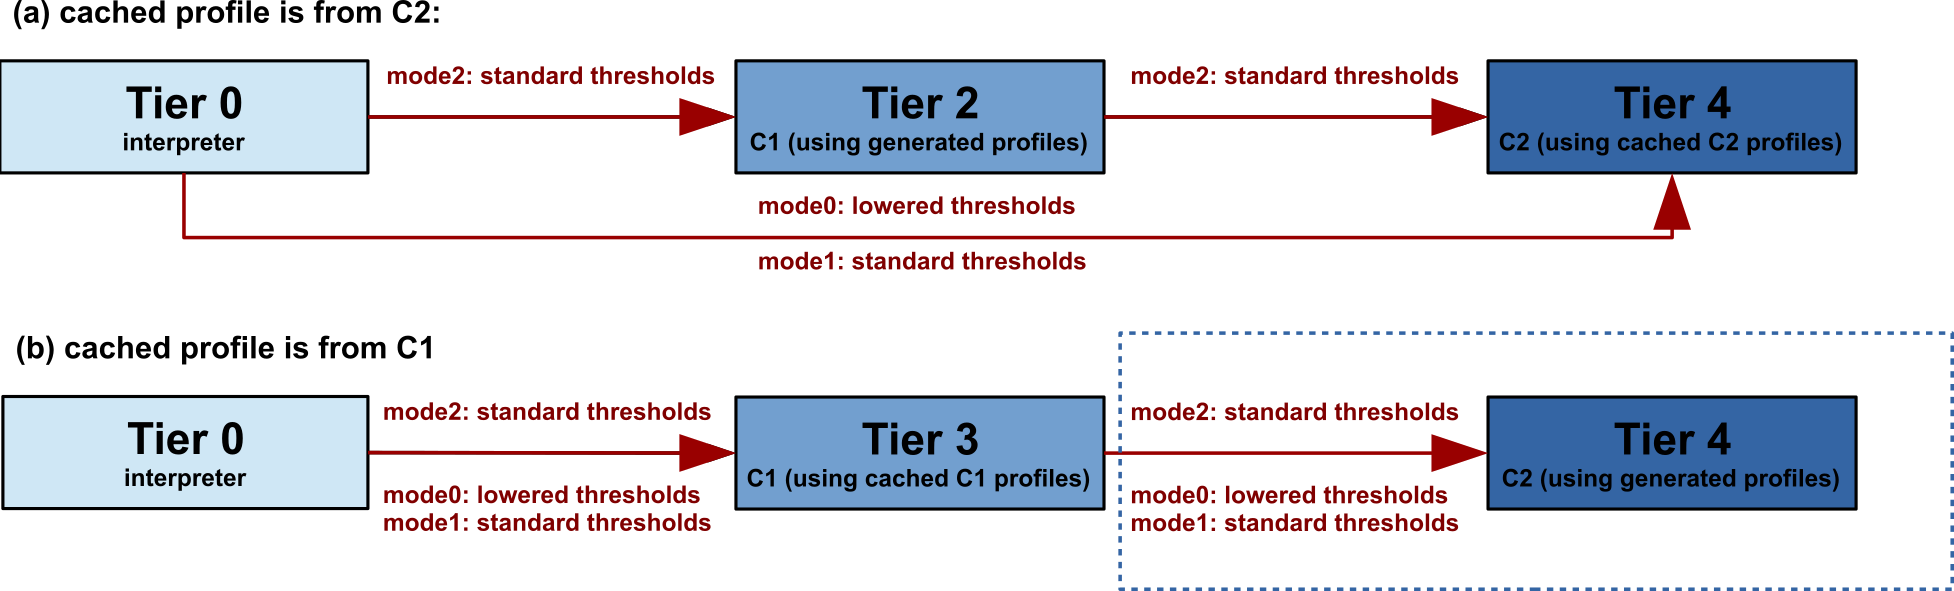
\includegraphics{figures/hs_tiers_threshold.png}
    \caption{Tier transitions of different modes}
    \label{f:hs_tiers_thresholds}
  \end{center}
\end{figure}


\section{Issues}
\label{s:issues}
If the profiles generated by multiple runs of the program deviate sharply it is likely that a cached profile does not fit to the current execution. In this case the compiled version would still trigger many deoptimizations and the method could end up having even worse performance since it's going to use the profile over and over again.
To circumvent that behavior I modified the code that only methods which have been deoptimized less then 10 times already will get compiled using cached profiles. If they are above that limit a standard compilation will be used instead.
The limit is 10 to allow a small number of recompilations. This could for example be useful when the method is deoptimized due to classes not being loaded. 
\section{Debug output}
\label{s:debugoutput}
For debugging and benchmarking purposes I implemented four debug flags that can be used along with \texttt{-XX:+CacheProfiles}.
\begin{table}[ht]
  \centering
 % \caption{}
  \label{t:debugflags}
  \begin{center}
    \begin{tabular}{| l | p{9.0cm} |}
       \hline
       \textbf{flag} & \textbf{description} \\ \hline\hline
       -XX:+PrintCacheProfiles & enable command line debug output for cached profiles\\ \hline
       -XX:+PrintDeoptimizationCount & prints amount of deoptimizations when the JVM gets shut down\\ \hline
       -XX:+PrintDeoptimizationCountVerbose & prints total the amount of deoptimizations on each deoptimization\\ \hline
       -XX:+PrintCompileQueueSize & prints the total amount of methods in the compile queue each time a method gets added \\ \hline
    \end{tabular}
  \end{center}
\end{table}

 
